% Options for packages loaded elsewhere
\PassOptionsToPackage{unicode}{hyperref}
\PassOptionsToPackage{hyphens}{url}
%
\documentclass[
]{article}
\usepackage{amsmath,amssymb}
\usepackage{iftex}
\ifPDFTeX
  \usepackage[T1]{fontenc}
  \usepackage[utf8]{inputenc}
  \usepackage{textcomp} % provide euro and other symbols
\else % if luatex or xetex
  \usepackage{unicode-math} % this also loads fontspec
  \defaultfontfeatures{Scale=MatchLowercase}
  \defaultfontfeatures[\rmfamily]{Ligatures=TeX,Scale=1}
\fi
\usepackage{lmodern}
\ifPDFTeX\else
  % xetex/luatex font selection
\fi
% Use upquote if available, for straight quotes in verbatim environments
\IfFileExists{upquote.sty}{\usepackage{upquote}}{}
\IfFileExists{microtype.sty}{% use microtype if available
  \usepackage[]{microtype}
  \UseMicrotypeSet[protrusion]{basicmath} % disable protrusion for tt fonts
}{}
\makeatletter
\@ifundefined{KOMAClassName}{% if non-KOMA class
  \IfFileExists{parskip.sty}{%
    \usepackage{parskip}
  }{% else
    \setlength{\parindent}{0pt}
    \setlength{\parskip}{6pt plus 2pt minus 1pt}}
}{% if KOMA class
  \KOMAoptions{parskip=half}}
\makeatother
\usepackage{xcolor}
\usepackage[margin=1in]{geometry}
\usepackage{longtable,booktabs,array}
\usepackage{calc} % for calculating minipage widths
% Correct order of tables after \paragraph or \subparagraph
\usepackage{etoolbox}
\makeatletter
\patchcmd\longtable{\par}{\if@noskipsec\mbox{}\fi\par}{}{}
\makeatother
% Allow footnotes in longtable head/foot
\IfFileExists{footnotehyper.sty}{\usepackage{footnotehyper}}{\usepackage{footnote}}
\makesavenoteenv{longtable}
\usepackage{graphicx}
\makeatletter
\newsavebox\pandoc@box
\newcommand*\pandocbounded[1]{% scales image to fit in text height/width
  \sbox\pandoc@box{#1}%
  \Gscale@div\@tempa{\textheight}{\dimexpr\ht\pandoc@box+\dp\pandoc@box\relax}%
  \Gscale@div\@tempb{\linewidth}{\wd\pandoc@box}%
  \ifdim\@tempb\p@<\@tempa\p@\let\@tempa\@tempb\fi% select the smaller of both
  \ifdim\@tempa\p@<\p@\scalebox{\@tempa}{\usebox\pandoc@box}%
  \else\usebox{\pandoc@box}%
  \fi%
}
% Set default figure placement to htbp
\def\fps@figure{htbp}
\makeatother
\setlength{\emergencystretch}{3em} % prevent overfull lines
\providecommand{\tightlist}{%
  \setlength{\itemsep}{0pt}\setlength{\parskip}{0pt}}
\setcounter{secnumdepth}{-\maxdimen} % remove section numbering
\usepackage{bookmark}
\IfFileExists{xurl.sty}{\usepackage{xurl}}{} % add URL line breaks if available
\urlstyle{same}
\hypersetup{
  hidelinks,
  pdfcreator={LaTeX via pandoc}}

\author{}
\date{\vspace{-2.5em}}

\begin{document}

\section{4주차 데이터 실험
집계}\label{uxc8fcuxcc28-uxb370uxc774uxd130-uxc2e4uxd5d8-uxc9d1uxacc4}

\subsection{실험의 목적}\label{uxc2e4uxd5d8uxc758-uxbaa9uxc801}

4주차 구글 예습 설문지 집계결과를 분석합니다.

Q1\textasciitilde Q6에서는 랜덤화의 효과로 Red, Black 이 얼마나 닮았는지
알아봅니다.

Q7에서는 부연설명을 어느 쪽에 붙이느냐에 따라서 Red 와 Black 의 응답이
달라지는 것을 알아봅니다.

끝으로 제출시간의 분포가 날마다 고른지, Red, Black 간에는 닮았는지
알아봅니다.

\subsubsection{Red, Black을 잘못 표시한
사람들}\label{red-blackuxc744-uxc798uxbabb-uxd45cuxc2dcuxd55c-uxc0acuxb78cuxb4e4}

\begin{longtable}[]{@{}
  >{\raggedright\arraybackslash}p{(\linewidth - 4\tabcolsep) * \real{0.3611}}
  >{\centering\arraybackslash}p{(\linewidth - 4\tabcolsep) * \real{0.2778}}
  >{\centering\arraybackslash}p{(\linewidth - 4\tabcolsep) * \real{0.3056}}@{}}
\toprule\noalign{}
\begin{minipage}[b]{\linewidth}\raggedright
~
\end{minipage} & \begin{minipage}[b]{\linewidth}\centering
Red(구글예습퀴즈)
\end{minipage} & \begin{minipage}[b]{\linewidth}\centering
Black(구글예습퀴즈)
\end{minipage} \\
\midrule\noalign{}
\endhead
\bottomrule\noalign{}
\endlastfoot
\textbf{Red(랜덤화출석부)} & 275 & 1 \\
\textbf{Black(랜덤화출석부)} & 3 & 285 \\
\textbf{계} & 278 & 286 \\
\end{longtable}

랜덤화출석부에 있는 Red, Black 과 실제 구글설문에 올린 Red, Black 이
다른 사람들의 수효는 4명입니다.

Red를 Black 이라고 한 사람이 1명, Black 을 Red 라고 한 사람이 3명입니다.

두 가지 방법으로 분석합니다.

우선 Red, Black 을 잘못 선택한 4명을 랜덤하게 둘로 나누면 어느 한 쪽
집단에 들어갈 기대인원은 4명을 둘로 나눈 2(명)이고, 표준오차는 4의
제곱근에 1/2을 곱해 준 1명이 됩니다.

실제로 Red를 Black 이라고 한 사람수, 1명이나 Black 을 Red 라고 한
사람수, 3명은 기대인원으로부터 표준오차 범위, 혹은 표준오차 두 배
범위에는 잘 들어갑니다.

두 번째 분석 방법은 확률을 계산해 보는 것입니다.

Red, Black 을 잘못 선택한 4명을 랜덤하게 둘로 나눌 때, 실제로 관찰된 3명
이상이나 1명이하로 잘못 선택한 사람수가 나올 가능성은 얼마나 되는가
입니다.

이 경우 공평한 동전던지기를 확률 법칙으로 표현한 이항분포로부터 계산할
수 있습니다.

시행횟수가 4이고 한 번 시행에서 성공확률이 1/2 인 이항분포에서
성공횟수가 1이하이거나 3이상을 관찰할 확률은 0.625입니다.

공평한 동전 던지기에서 앞면이 1개 이하 나오는 확률은 3개 이상 나오는
확률과 같기 때문에 사실상 한쪽만 계산해서 2배 해 주면 됩니다.

이 값을 p-value 라고 하는데, p-value가 0.05보다 작을 때
\textbf{통계적으로 유의한 차이를 관찰}하였다고 말합니다.

즉, 공평한 동전을 던지는 것과 같은 과정이라고 가정하였을 때 실제로
관찰된 값들이 가정으로부터 얼마나 떨어져 있는지를 표현한 것입니다.

0.05는 이런 실험을 스무 번 정도 반복하면 1번 나올 정도로 드문 사건을
의미합니다.

즉 가정이 잘못되었다는 것입니다.

그런데 Red, Black 을 잘못 표시한 사람들의 분포에서 관찰된 p-value 는
0.05와는 비교도 안될 정도로 큰 값입니다.

따라서 두 집단이 랜덤화 효과가 작동하여 \textbf{통계적으로 유의한 차이를
보이지 않는다}고 할 수 있습니다.

\subsubsection{응답인원의 Red,
Black}\label{uxc751uxb2f5uxc778uxc6d0uxc758-red-black}

Red 로 응답한 인원은 278명, Black 에 응답한 인원은 286명입니다.

전체 응답인원 564 명을 랜덤하게 둘로 나눌 때 어느 한 쪽의 기대인원은
전체 응답인원의 절반인 282명이고, 표준오차는 전체 응답인원의 제곱근에
1/2을 곱해 준 11.9 명입니다.

따라서 Red, Black 각 그룹에 관찰된 인원은 기대인원으로부터 표준오차
범위, 혹은 2배의 표준오차 범위 안에 들어갑니다.

\subsection{Q1. 세종대왕 시대
조세제도}\label{q1.-uxc138uxc885uxb300uxc655-uxc2dcuxb300-uxc870uxc138uxc81cuxb3c4}

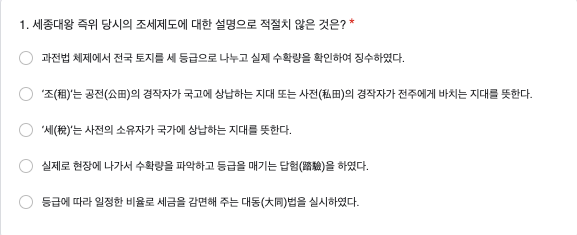
\includegraphics[width=0.75\linewidth]{./pics/Quiz230322_Q1}

\subsubsection{조선초기
조세제도}\label{uxc870uxc120uxcd08uxae30-uxc870uxc138uxc81cuxb3c4}

\begin{longtable}[]{@{}
  >{\raggedright\arraybackslash}p{(\linewidth - 12\tabcolsep) * \real{0.0674}}
  >{\centering\arraybackslash}p{(\linewidth - 12\tabcolsep) * \real{0.1854}}
  >{\centering\arraybackslash}p{(\linewidth - 12\tabcolsep) * \real{0.1854}}
  >{\centering\arraybackslash}p{(\linewidth - 12\tabcolsep) * \real{0.1854}}
  >{\centering\arraybackslash}p{(\linewidth - 12\tabcolsep) * \real{0.1798}}
  >{\centering\arraybackslash}p{(\linewidth - 12\tabcolsep) * \real{0.1629}}
  >{\centering\arraybackslash}p{(\linewidth - 12\tabcolsep) * \real{0.0337}}@{}}
\toprule\noalign{}
\begin{minipage}[b]{\linewidth}\raggedright
~
\end{minipage} & \begin{minipage}[b]{\linewidth}\centering
과전법 체제에서 전국 토지를 세 등급으로 나누고 실제 수확량을 확인하여
징수하였다.
\end{minipage} & \begin{minipage}[b]{\linewidth}\centering
'조(租)'는 공전(公田)의 경작자가 국고에 상납하는 지대 또는 사전(私田)의
경작자가 전주에게 바치는 지대를 뜻한다.
\end{minipage} & \begin{minipage}[b]{\linewidth}\centering
'세(稅)'는 사전의 소유자가 국가에 상납하는 지세를 뜻한다.
\end{minipage} & \begin{minipage}[b]{\linewidth}\centering
실제로 현장에 나가서 수확량을 파악하고 등급을 매기는 답험(踏驗)을
하였다.
\end{minipage} & \begin{minipage}[b]{\linewidth}\centering
등급에 따라 일정한 비율로 세금을 감면해 주는 대동(大同)법을 실시하였다.
\end{minipage} & \begin{minipage}[b]{\linewidth}\centering
계
\end{minipage} \\
\midrule\noalign{}
\endhead
\bottomrule\noalign{}
\endlastfoot
\textbf{Red} & 22 & 28 & 26 & 22 & 180 & 278 \\
\textbf{Black} & 17 & 30 & 17 & 19 & 203 & 286 \\
\textbf{계} & 39 & 58 & 43 & 41 & 383 & 564 \\
\end{longtable}

\begin{longtable}[]{@{}
  >{\raggedleft\arraybackslash}p{(\linewidth - 4\tabcolsep) * \real{0.2361}}
  >{\raggedleft\arraybackslash}p{(\linewidth - 4\tabcolsep) * \real{0.0694}}
  >{\raggedleft\arraybackslash}p{(\linewidth - 4\tabcolsep) * \real{0.1389}}@{}}
\caption{Pearson's Chi-squared test: \texttt{.}}\tabularnewline
\toprule\noalign{}
\begin{minipage}[b]{\linewidth}\raggedleft
Test statistic
\end{minipage} & \begin{minipage}[b]{\linewidth}\raggedleft
df
\end{minipage} & \begin{minipage}[b]{\linewidth}\raggedleft
P value
\end{minipage} \\
\midrule\noalign{}
\endfirsthead
\toprule\noalign{}
\begin{minipage}[b]{\linewidth}\raggedleft
Test statistic
\end{minipage} & \begin{minipage}[b]{\linewidth}\raggedleft
df
\end{minipage} & \begin{minipage}[b]{\linewidth}\raggedleft
P value
\end{minipage} \\
\midrule\noalign{}
\endhead
\bottomrule\noalign{}
\endlastfoot
4.082 & 4 & 0.3951 \\
\end{longtable}

Q1의 집계 결과가 Red, Black 간에 통계적으로 유의한 차이가 있는지
알아보기 위하여 카이제곱 테스트를 수행하였습니다.

그 결과 카이제곱 통계량은 4.08, 자유도는 4 , p-value 는 0.3951이므로
Red, Black 간에 통계적으로 유의한 차이를 보이지 않습니다.

실제로 닮은 게 느껴집니까?

\subsubsection{조선초기
조세제도(\%)}\label{uxc870uxc120uxcd08uxae30-uxc870uxc138uxc81cuxb3c4-1}

\begin{longtable}[]{@{}
  >{\centering\arraybackslash}p{(\linewidth - 10\tabcolsep) * \real{0.1964}}
  >{\centering\arraybackslash}p{(\linewidth - 10\tabcolsep) * \real{0.1964}}
  >{\centering\arraybackslash}p{(\linewidth - 10\tabcolsep) * \real{0.1964}}
  >{\centering\arraybackslash}p{(\linewidth - 10\tabcolsep) * \real{0.1905}}
  >{\centering\arraybackslash}p{(\linewidth - 10\tabcolsep) * \real{0.1726}}
  >{\centering\arraybackslash}p{(\linewidth - 10\tabcolsep) * \real{0.0476}}@{}}
\toprule\noalign{}
\begin{minipage}[b]{\linewidth}\centering
과전법 체제에서 전국 토지를 세 등급으로 나누고 실제 수확량을 확인하여
징수하였다.
\end{minipage} & \begin{minipage}[b]{\linewidth}\centering
'조(租)'는 공전(公田)의 경작자가 국고에 상납하는 지대 또는 사전(私田)의
경작자가 전주에게 바치는 지대를 뜻한다.
\end{minipage} & \begin{minipage}[b]{\linewidth}\centering
'세(稅)'는 사전의 소유자가 국가에 상납하는 지세를 뜻한다.
\end{minipage} & \begin{minipage}[b]{\linewidth}\centering
실제로 현장에 나가서 수확량을 파악하고 등급을 매기는 답험(踏驗)을
하였다.
\end{minipage} & \begin{minipage}[b]{\linewidth}\centering
등급에 따라 일정한 비율로 세금을 감면해 주는 대동(大同)법을 실시하였다.
\end{minipage} & \begin{minipage}[b]{\linewidth}\centering
계
\end{minipage} \\
\midrule\noalign{}
\endhead
\bottomrule\noalign{}
\endlastfoot
6.9 & 10.3 & 7.6 & 7.3 & 67.9 & 100.0 \\
\end{longtable}

정답률은 Red, Black 을 합하여 계산하는데, 67.9(\%) 입니다.

\subsection{Q2. 공법도입에 대한 대신들의
찬성율}\label{q2.-uxacf5uxbc95uxb3c4uxc785uxc5d0-uxb300uxd55c-uxb300uxc2e0uxb4e4uxc758-uxcc2cuxc131uxc728}

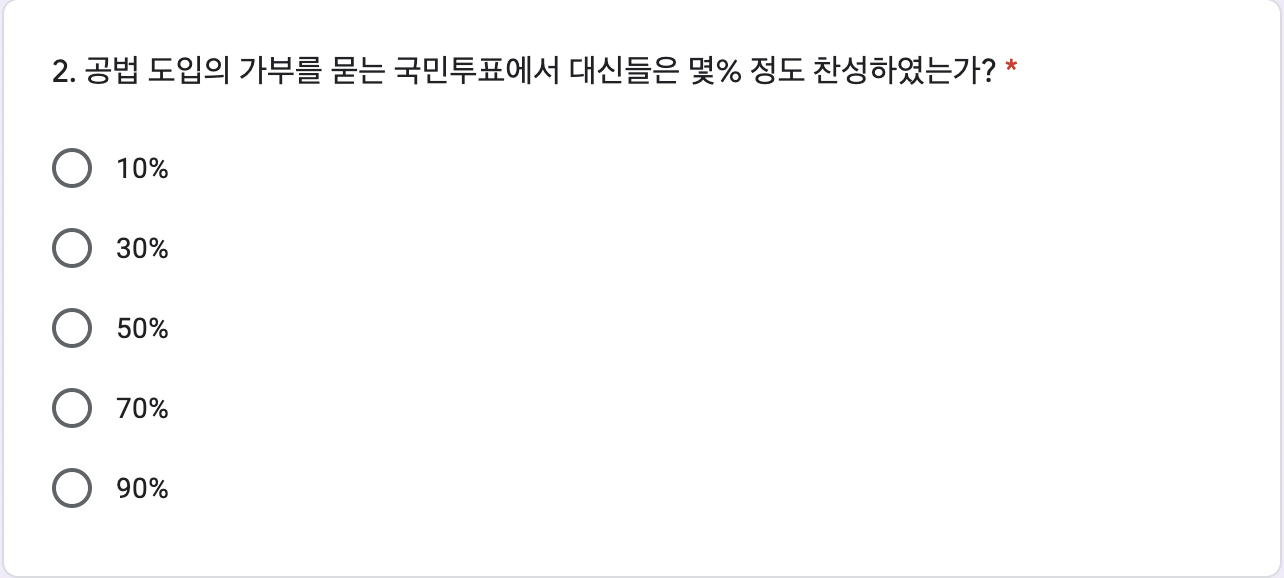
\includegraphics[width=0.75\linewidth]{./pics/Quiz210913_Q2}

\subsubsection{공법도입과
대신들(집계표)}\label{uxacf5uxbc95uxb3c4uxc785uxacfc-uxb300uxc2e0uxb4e4uxc9d1uxacc4uxd45c}

\begin{longtable}[]{@{}
  >{\raggedright\arraybackslash}p{(\linewidth - 12\tabcolsep) * \real{0.1667}}
  >{\raggedleft\arraybackslash}p{(\linewidth - 12\tabcolsep) * \real{0.0833}}
  >{\raggedleft\arraybackslash}p{(\linewidth - 12\tabcolsep) * \real{0.0833}}
  >{\raggedleft\arraybackslash}p{(\linewidth - 12\tabcolsep) * \real{0.0833}}
  >{\raggedleft\arraybackslash}p{(\linewidth - 12\tabcolsep) * \real{0.0833}}
  >{\raggedleft\arraybackslash}p{(\linewidth - 12\tabcolsep) * \real{0.0833}}
  >{\centering\arraybackslash}p{(\linewidth - 12\tabcolsep) * \real{0.0833}}@{}}
\toprule\noalign{}
\begin{minipage}[b]{\linewidth}\raggedright
~
\end{minipage} & \begin{minipage}[b]{\linewidth}\raggedleft
10\%
\end{minipage} & \begin{minipage}[b]{\linewidth}\raggedleft
30\%
\end{minipage} & \begin{minipage}[b]{\linewidth}\raggedleft
50\%
\end{minipage} & \begin{minipage}[b]{\linewidth}\raggedleft
70\%
\end{minipage} & \begin{minipage}[b]{\linewidth}\raggedleft
90\%
\end{minipage} & \begin{minipage}[b]{\linewidth}\centering
계
\end{minipage} \\
\midrule\noalign{}
\endhead
\bottomrule\noalign{}
\endlastfoot
\textbf{Red} & 153 & 54 & 28 & 27 & 16 & 278 \\
\textbf{Black} & 160 & 46 & 26 & 32 & 22 & 286 \\
\textbf{계} & 313 & 100 & 54 & 59 & 38 & 564 \\
\end{longtable}

\begin{longtable}[]{@{}
  >{\raggedleft\arraybackslash}p{(\linewidth - 4\tabcolsep) * \real{0.2361}}
  >{\raggedleft\arraybackslash}p{(\linewidth - 4\tabcolsep) * \real{0.0694}}
  >{\raggedleft\arraybackslash}p{(\linewidth - 4\tabcolsep) * \real{0.1389}}@{}}
\caption{Pearson's Chi-squared test: \texttt{.}}\tabularnewline
\toprule\noalign{}
\begin{minipage}[b]{\linewidth}\raggedleft
Test statistic
\end{minipage} & \begin{minipage}[b]{\linewidth}\raggedleft
df
\end{minipage} & \begin{minipage}[b]{\linewidth}\raggedleft
P value
\end{minipage} \\
\midrule\noalign{}
\endfirsthead
\toprule\noalign{}
\begin{minipage}[b]{\linewidth}\raggedleft
Test statistic
\end{minipage} & \begin{minipage}[b]{\linewidth}\raggedleft
df
\end{minipage} & \begin{minipage}[b]{\linewidth}\raggedleft
P value
\end{minipage} \\
\midrule\noalign{}
\endhead
\bottomrule\noalign{}
\endlastfoot
2.129 & 4 & 0.7121 \\
\end{longtable}

Q2의 집계 결과가 Red, Black 간에 통계적으로 유의한 차이가 있는지
알아보기 위하여 카이제곱 테스트를 수행하였습니다.

그 결과 카이제곱 통계량은 2.129, 자유도는 4, p-value 는 0.7121이므로
Red, Black 간에 통계적으로 유의한 차이를 보이지 않습니다.

실제로 닮은 게 느껴집니까?

\subsubsection{공법도입과
대신들(\%)}\label{uxacf5uxbc95uxb3c4uxc785uxacfc-uxb300uxc2e0uxb4e4}

\begin{longtable}[]{@{}
  >{\raggedleft\arraybackslash}p{(\linewidth - 10\tabcolsep) * \real{0.0972}}
  >{\raggedleft\arraybackslash}p{(\linewidth - 10\tabcolsep) * \real{0.0972}}
  >{\raggedleft\arraybackslash}p{(\linewidth - 10\tabcolsep) * \real{0.0833}}
  >{\raggedleft\arraybackslash}p{(\linewidth - 10\tabcolsep) * \real{0.0972}}
  >{\raggedleft\arraybackslash}p{(\linewidth - 10\tabcolsep) * \real{0.0833}}
  >{\centering\arraybackslash}p{(\linewidth - 10\tabcolsep) * \real{0.1111}}@{}}
\toprule\noalign{}
\begin{minipage}[b]{\linewidth}\raggedleft
10\%
\end{minipage} & \begin{minipage}[b]{\linewidth}\raggedleft
30\%
\end{minipage} & \begin{minipage}[b]{\linewidth}\raggedleft
50\%
\end{minipage} & \begin{minipage}[b]{\linewidth}\raggedleft
70\%
\end{minipage} & \begin{minipage}[b]{\linewidth}\raggedleft
90\%
\end{minipage} & \begin{minipage}[b]{\linewidth}\centering
계
\end{minipage} \\
\midrule\noalign{}
\endhead
\bottomrule\noalign{}
\endlastfoot
55.5 & 17.7 & 9.6 & 10.5 & 6.7 & 100.0 \\
\end{longtable}

정답률은 Red, Black 을 합하여 계산하는데, 55.5(\%) 입니다.

\subsection{Q3. 공법도입과 품관촌민들의
찬반}\label{q3.-uxacf5uxbc95uxb3c4uxc785uxacfc-uxd488uxad00uxcd0cuxbbfcuxb4e4uxc758-uxcc2cuxbc18}

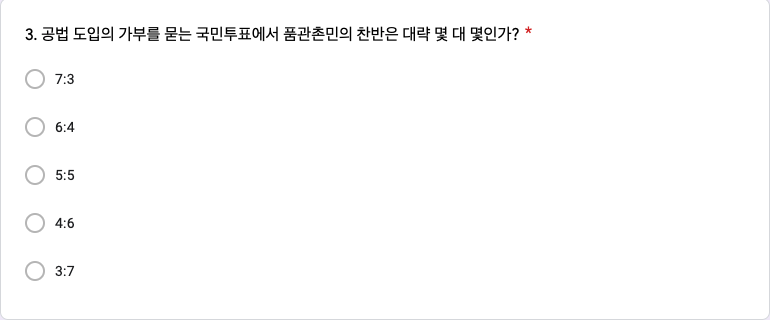
\includegraphics[width=0.75\linewidth]{./pics/Quiz210316_Q3}

\subsubsection{품관촌민들의
찬반(집계표)}\label{uxd488uxad00uxcd0cuxbbfcuxb4e4uxc758-uxcc2cuxbc18uxc9d1uxacc4uxd45c}

\begin{longtable}[]{@{}
  >{\raggedright\arraybackslash}p{(\linewidth - 12\tabcolsep) * \real{0.1667}}
  >{\raggedleft\arraybackslash}p{(\linewidth - 12\tabcolsep) * \real{0.0833}}
  >{\raggedleft\arraybackslash}p{(\linewidth - 12\tabcolsep) * \real{0.0833}}
  >{\raggedleft\arraybackslash}p{(\linewidth - 12\tabcolsep) * \real{0.0833}}
  >{\raggedleft\arraybackslash}p{(\linewidth - 12\tabcolsep) * \real{0.0833}}
  >{\raggedleft\arraybackslash}p{(\linewidth - 12\tabcolsep) * \real{0.0833}}
  >{\centering\arraybackslash}p{(\linewidth - 12\tabcolsep) * \real{0.0833}}@{}}
\toprule\noalign{}
\begin{minipage}[b]{\linewidth}\raggedright
~
\end{minipage} & \begin{minipage}[b]{\linewidth}\raggedleft
7:3
\end{minipage} & \begin{minipage}[b]{\linewidth}\raggedleft
6:4
\end{minipage} & \begin{minipage}[b]{\linewidth}\raggedleft
5:5
\end{minipage} & \begin{minipage}[b]{\linewidth}\raggedleft
4:6
\end{minipage} & \begin{minipage}[b]{\linewidth}\raggedleft
3:7
\end{minipage} & \begin{minipage}[b]{\linewidth}\centering
계
\end{minipage} \\
\midrule\noalign{}
\endhead
\bottomrule\noalign{}
\endlastfoot
\textbf{Red} & 48 & 159 & 25 & 22 & 24 & 278 \\
\textbf{Black} & 62 & 162 & 25 & 18 & 19 & 286 \\
\textbf{계} & 110 & 321 & 50 & 40 & 43 & 564 \\
\end{longtable}

\begin{longtable}[]{@{}
  >{\raggedleft\arraybackslash}p{(\linewidth - 4\tabcolsep) * \real{0.2361}}
  >{\raggedleft\arraybackslash}p{(\linewidth - 4\tabcolsep) * \real{0.0694}}
  >{\raggedleft\arraybackslash}p{(\linewidth - 4\tabcolsep) * \real{0.1389}}@{}}
\caption{Pearson's Chi-squared test: \texttt{.}}\tabularnewline
\toprule\noalign{}
\begin{minipage}[b]{\linewidth}\raggedleft
Test statistic
\end{minipage} & \begin{minipage}[b]{\linewidth}\raggedleft
df
\end{minipage} & \begin{minipage}[b]{\linewidth}\raggedleft
P value
\end{minipage} \\
\midrule\noalign{}
\endfirsthead
\toprule\noalign{}
\begin{minipage}[b]{\linewidth}\raggedleft
Test statistic
\end{minipage} & \begin{minipage}[b]{\linewidth}\raggedleft
df
\end{minipage} & \begin{minipage}[b]{\linewidth}\raggedleft
P value
\end{minipage} \\
\midrule\noalign{}
\endhead
\bottomrule\noalign{}
\endlastfoot
2.678 & 4 & 0.613 \\
\end{longtable}

Q3의 집계 결과가 Red, Black 간에 통계적으로 유의한 차이가 있는지
알아보기 위하여 카이제곱 테스트를 수행하였습니다.

그 결과 카이제곱 통계량은 2.678, 자유도는 4, p-value 는 0.6130이므로
Red, Black 간에 통계적으로 유의한 차이를 보이지 않습니다.

실제로 닮은 게 느껴집니까?

\subsubsection{품관촌민들의
찬반(\%)}\label{uxd488uxad00uxcd0cuxbbfcuxb4e4uxc758-uxcc2cuxbc18}

\begin{longtable}[]{@{}
  >{\raggedleft\arraybackslash}p{(\linewidth - 10\tabcolsep) * \real{0.0972}}
  >{\raggedleft\arraybackslash}p{(\linewidth - 10\tabcolsep) * \real{0.0972}}
  >{\raggedleft\arraybackslash}p{(\linewidth - 10\tabcolsep) * \real{0.0833}}
  >{\raggedleft\arraybackslash}p{(\linewidth - 10\tabcolsep) * \real{0.0833}}
  >{\raggedleft\arraybackslash}p{(\linewidth - 10\tabcolsep) * \real{0.0833}}
  >{\centering\arraybackslash}p{(\linewidth - 10\tabcolsep) * \real{0.1111}}@{}}
\toprule\noalign{}
\begin{minipage}[b]{\linewidth}\raggedleft
7:3
\end{minipage} & \begin{minipage}[b]{\linewidth}\raggedleft
6:4
\end{minipage} & \begin{minipage}[b]{\linewidth}\raggedleft
5:5
\end{minipage} & \begin{minipage}[b]{\linewidth}\raggedleft
4:6
\end{minipage} & \begin{minipage}[b]{\linewidth}\raggedleft
3:7
\end{minipage} & \begin{minipage}[b]{\linewidth}\centering
계
\end{minipage} \\
\midrule\noalign{}
\endhead
\bottomrule\noalign{}
\endlastfoot
19.5 & 56.9 & 8.9 & 7.1 & 7.6 & 100.0 \\
\end{longtable}

정답률은 Red, Black 을 합하여 계산하는데, 56.9(\%) 입니다.

\subsection{Q4. 공법}\label{q4.-uxacf5uxbc95}

\begin{flushleft}
\includegraphics[width=0.75\linewidth]{./pics/Quiz210316_Q4} \end{flushleft}

\subsubsection{기본세율}\label{uxae30uxbcf8uxc138uxc728}

\begin{longtable}[]{@{}
  >{\raggedright\arraybackslash}p{(\linewidth - 10\tabcolsep) * \real{0.1667}}
  >{\raggedleft\arraybackslash}p{(\linewidth - 10\tabcolsep) * \real{0.0972}}
  >{\raggedleft\arraybackslash}p{(\linewidth - 10\tabcolsep) * \real{0.0972}}
  >{\raggedleft\arraybackslash}p{(\linewidth - 10\tabcolsep) * \real{0.0972}}
  >{\raggedleft\arraybackslash}p{(\linewidth - 10\tabcolsep) * \real{0.0972}}
  >{\centering\arraybackslash}p{(\linewidth - 10\tabcolsep) * \real{0.0972}}@{}}
\toprule\noalign{}
\begin{minipage}[b]{\linewidth}\raggedright
~
\end{minipage} & \begin{minipage}[b]{\linewidth}\raggedleft
1/10
\end{minipage} & \begin{minipage}[b]{\linewidth}\raggedleft
1/15
\end{minipage} & \begin{minipage}[b]{\linewidth}\raggedleft
1/20
\end{minipage} & \begin{minipage}[b]{\linewidth}\raggedleft
1/30
\end{minipage} & \begin{minipage}[b]{\linewidth}\centering
계
\end{minipage} \\
\midrule\noalign{}
\endhead
\bottomrule\noalign{}
\endlastfoot
\textbf{Red} & 84 & 47 & 132 & 15 & 278 \\
\textbf{Black} & 88 & 29 & 154 & 15 & 286 \\
\textbf{계} & 172 & 76 & 286 & 30 & 564 \\
\end{longtable}

\begin{longtable}[]{@{}
  >{\raggedleft\arraybackslash}p{(\linewidth - 4\tabcolsep) * \real{0.2361}}
  >{\raggedleft\arraybackslash}p{(\linewidth - 4\tabcolsep) * \real{0.0694}}
  >{\raggedleft\arraybackslash}p{(\linewidth - 4\tabcolsep) * \real{0.1389}}@{}}
\caption{Pearson's Chi-squared test: \texttt{.}}\tabularnewline
\toprule\noalign{}
\begin{minipage}[b]{\linewidth}\raggedleft
Test statistic
\end{minipage} & \begin{minipage}[b]{\linewidth}\raggedleft
df
\end{minipage} & \begin{minipage}[b]{\linewidth}\raggedleft
P value
\end{minipage} \\
\midrule\noalign{}
\endfirsthead
\toprule\noalign{}
\begin{minipage}[b]{\linewidth}\raggedleft
Test statistic
\end{minipage} & \begin{minipage}[b]{\linewidth}\raggedleft
df
\end{minipage} & \begin{minipage}[b]{\linewidth}\raggedleft
P value
\end{minipage} \\
\midrule\noalign{}
\endhead
\bottomrule\noalign{}
\endlastfoot
5.936 & 3 & 0.1148 \\
\end{longtable}

Q4의 집계 결과가 Red, Black 간에 통계적으로 유의한 차이가 있는지
알아보기 위하여 카이제곱 테스트를 수행하였습니다.

그 결과 카이제곱 통계량은 5.936, 자유도는 3, p-value 는 0.1148이므로
Red, Black 간에 통계적으로 유의한 차이를 보이지 않습니다.

실제로 닮은 게 느껴집니까?

\subsubsection{기본세율(\%)}\label{uxae30uxbcf8uxc138uxc728-1}

\begin{longtable}[]{@{}
  >{\raggedleft\arraybackslash}p{(\linewidth - 8\tabcolsep) * \real{0.0972}}
  >{\raggedleft\arraybackslash}p{(\linewidth - 8\tabcolsep) * \real{0.0972}}
  >{\raggedleft\arraybackslash}p{(\linewidth - 8\tabcolsep) * \real{0.0972}}
  >{\raggedleft\arraybackslash}p{(\linewidth - 8\tabcolsep) * \real{0.0972}}
  >{\centering\arraybackslash}p{(\linewidth - 8\tabcolsep) * \real{0.1111}}@{}}
\toprule\noalign{}
\begin{minipage}[b]{\linewidth}\raggedleft
1/10
\end{minipage} & \begin{minipage}[b]{\linewidth}\raggedleft
1/15
\end{minipage} & \begin{minipage}[b]{\linewidth}\raggedleft
1/20
\end{minipage} & \begin{minipage}[b]{\linewidth}\raggedleft
1/30
\end{minipage} & \begin{minipage}[b]{\linewidth}\centering
계
\end{minipage} \\
\midrule\noalign{}
\endhead
\bottomrule\noalign{}
\endlastfoot
30.5 & 13.5 & 50.7 & 5.3 & 100.0 \\
\end{longtable}

정답률은 Red, Black 을 합하여 계산하는데, 30.5(\%) 입니다.

\subsection{Q5. 1423년 조선시대 호구와
인구}\label{q5.-1423uxb144-uxc870uxc120uxc2dcuxb300-uxd638uxad6cuxc640-uxc778uxad6c}

\begin{flushleft}
\includegraphics[width=0.75\linewidth]{./pics/Quiz210316_Q5} \end{flushleft}

\subsubsection{호구와 인구}\label{uxd638uxad6cuxc640-uxc778uxad6c}

\begin{longtable}[]{@{}
  >{\raggedright\arraybackslash}p{(\linewidth - 10\tabcolsep) * \real{0.1667}}
  >{\centering\arraybackslash}p{(\linewidth - 10\tabcolsep) * \real{0.1250}}
  >{\centering\arraybackslash}p{(\linewidth - 10\tabcolsep) * \real{0.1250}}
  >{\centering\arraybackslash}p{(\linewidth - 10\tabcolsep) * \real{0.1250}}
  >{\centering\arraybackslash}p{(\linewidth - 10\tabcolsep) * \real{0.1389}}
  >{\centering\arraybackslash}p{(\linewidth - 10\tabcolsep) * \real{0.0833}}@{}}
\toprule\noalign{}
\begin{minipage}[b]{\linewidth}\raggedright
~
\end{minipage} & \begin{minipage}[b]{\linewidth}\centering
15만호
\end{minipage} & \begin{minipage}[b]{\linewidth}\centering
20만호
\end{minipage} & \begin{minipage}[b]{\linewidth}\centering
44만호
\end{minipage} & \begin{minipage}[b]{\linewidth}\centering
130만호
\end{minipage} & \begin{minipage}[b]{\linewidth}\centering
계
\end{minipage} \\
\midrule\noalign{}
\endhead
\bottomrule\noalign{}
\endlastfoot
\textbf{Red} & 11 & 164 & 87 & 16 & 278 \\
\textbf{Black} & 22 & 151 & 105 & 8 & 286 \\
\textbf{계} & 33 & 315 & 192 & 24 & 564 \\
\end{longtable}

\begin{longtable}[]{@{}
  >{\raggedleft\arraybackslash}p{(\linewidth - 4\tabcolsep) * \real{0.2361}}
  >{\raggedleft\arraybackslash}p{(\linewidth - 4\tabcolsep) * \real{0.0694}}
  >{\raggedleft\arraybackslash}p{(\linewidth - 4\tabcolsep) * \real{0.1667}}@{}}
\caption{Pearson's Chi-squared test: \texttt{.}}\tabularnewline
\toprule\noalign{}
\begin{minipage}[b]{\linewidth}\raggedleft
Test statistic
\end{minipage} & \begin{minipage}[b]{\linewidth}\raggedleft
df
\end{minipage} & \begin{minipage}[b]{\linewidth}\raggedleft
P value
\end{minipage} \\
\midrule\noalign{}
\endfirsthead
\toprule\noalign{}
\begin{minipage}[b]{\linewidth}\raggedleft
Test statistic
\end{minipage} & \begin{minipage}[b]{\linewidth}\raggedleft
df
\end{minipage} & \begin{minipage}[b]{\linewidth}\raggedleft
P value
\end{minipage} \\
\midrule\noalign{}
\endhead
\bottomrule\noalign{}
\endlastfoot
8.446 & 3 & 0.03765 * \\
\end{longtable}

Q5의 집계 결과가 Red, Black 간에 통계적으로 유의한 차이가 있는지
알아보기 위하여 카이제곱 테스트를 수행하였습니다.

그 결과 카이제곱 통계량은 8.446, 자유도는 3, p-value 는 0.0376이므로
Red, Black 간에 통계적으로 유의한 차이를 보이고 있습니다.

\subsubsection{호구와 인구(\%)}\label{uxd638uxad6cuxc640-uxc778uxad6c-1}

\begin{longtable}[]{@{}
  >{\centering\arraybackslash}p{(\linewidth - 8\tabcolsep) * \real{0.1250}}
  >{\centering\arraybackslash}p{(\linewidth - 8\tabcolsep) * \real{0.1250}}
  >{\centering\arraybackslash}p{(\linewidth - 8\tabcolsep) * \real{0.1250}}
  >{\centering\arraybackslash}p{(\linewidth - 8\tabcolsep) * \real{0.1389}}
  >{\centering\arraybackslash}p{(\linewidth - 8\tabcolsep) * \real{0.1389}}@{}}
\toprule\noalign{}
\begin{minipage}[b]{\linewidth}\centering
15만호
\end{minipage} & \begin{minipage}[b]{\linewidth}\centering
20만호
\end{minipage} & \begin{minipage}[b]{\linewidth}\centering
44만호
\end{minipage} & \begin{minipage}[b]{\linewidth}\centering
130만호
\end{minipage} & \begin{minipage}[b]{\linewidth}\centering
계
\end{minipage} \\
\midrule\noalign{}
\endhead
\bottomrule\noalign{}
\endlastfoot
5.9 & 55.9 & 34.0 & 4.3 & 100.0 \\
\end{longtable}

정답률은 Red, Black 을 합하여 계산하는데, 55.9(\%) 입니다.

\subsection{Q6. 지방관료와
품관촌민}\label{q6.-uxc9c0uxbc29uxad00uxb8ccuxc640-uxd488uxad00uxcd0cuxbbfc}

\begin{flushleft}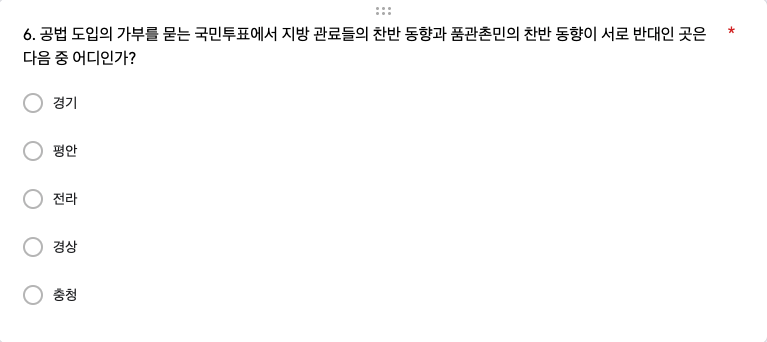
\includegraphics[width=0.75\linewidth]{./pics/Quiz210316_Q6} \end{flushleft}

\subsubsection{찬반이 반대인
곳(집계표)}\label{uxcc2cuxbc18uxc774-uxbc18uxb300uxc778-uxacf3uxc9d1uxacc4uxd45c}

\begin{longtable}[]{@{}
  >{\raggedright\arraybackslash}p{(\linewidth - 12\tabcolsep) * \real{0.1667}}
  >{\centering\arraybackslash}p{(\linewidth - 12\tabcolsep) * \real{0.0972}}
  >{\centering\arraybackslash}p{(\linewidth - 12\tabcolsep) * \real{0.0972}}
  >{\centering\arraybackslash}p{(\linewidth - 12\tabcolsep) * \real{0.0972}}
  >{\centering\arraybackslash}p{(\linewidth - 12\tabcolsep) * \real{0.0972}}
  >{\centering\arraybackslash}p{(\linewidth - 12\tabcolsep) * \real{0.0972}}
  >{\centering\arraybackslash}p{(\linewidth - 12\tabcolsep) * \real{0.0972}}@{}}
\toprule\noalign{}
\begin{minipage}[b]{\linewidth}\raggedright
~
\end{minipage} & \begin{minipage}[b]{\linewidth}\centering
경기
\end{minipage} & \begin{minipage}[b]{\linewidth}\centering
평안
\end{minipage} & \begin{minipage}[b]{\linewidth}\centering
전라
\end{minipage} & \begin{minipage}[b]{\linewidth}\centering
경상
\end{minipage} & \begin{minipage}[b]{\linewidth}\centering
충청
\end{minipage} & \begin{minipage}[b]{\linewidth}\centering
계
\end{minipage} \\
\midrule\noalign{}
\endhead
\bottomrule\noalign{}
\endlastfoot
\textbf{Red} & 25 & 39 & 44 & 40 & 130 & 278 \\
\textbf{Black} & 25 & 37 & 51 & 43 & 130 & 286 \\
\textbf{계} & 50 & 76 & 95 & 83 & 260 & 564 \\
\end{longtable}

\begin{longtable}[]{@{}
  >{\raggedleft\arraybackslash}p{(\linewidth - 4\tabcolsep) * \real{0.2361}}
  >{\raggedleft\arraybackslash}p{(\linewidth - 4\tabcolsep) * \real{0.0694}}
  >{\raggedleft\arraybackslash}p{(\linewidth - 4\tabcolsep) * \real{0.1389}}@{}}
\caption{Pearson's Chi-squared test: \texttt{.}}\tabularnewline
\toprule\noalign{}
\begin{minipage}[b]{\linewidth}\raggedleft
Test statistic
\end{minipage} & \begin{minipage}[b]{\linewidth}\raggedleft
df
\end{minipage} & \begin{minipage}[b]{\linewidth}\raggedleft
P value
\end{minipage} \\
\midrule\noalign{}
\endfirsthead
\toprule\noalign{}
\begin{minipage}[b]{\linewidth}\raggedleft
Test statistic
\end{minipage} & \begin{minipage}[b]{\linewidth}\raggedleft
df
\end{minipage} & \begin{minipage}[b]{\linewidth}\raggedleft
P value
\end{minipage} \\
\midrule\noalign{}
\endhead
\bottomrule\noalign{}
\endlastfoot
0.5635 & 4 & 0.967 \\
\end{longtable}

Q6의 집계 결과가 Red, Black 간에 통계적으로 유의한 차이가 있는지
알아보기 위하여 카이제곱 테스트를 수행하였습니다.

그 결과 카이제곱 통계량은 0.563, 자유도는 4, p-value 는 0.9670이므로
Red, Black 간에 통계적으로 유의한 차이를 보이지 않습니다.

실제로 닮은 게 느껴집니까?

\subsubsection{찬반이 반대인
곳(\%)}\label{uxcc2cuxbc18uxc774-uxbc18uxb300uxc778-uxacf3}

\begin{longtable}[]{@{}
  >{\centering\arraybackslash}p{(\linewidth - 10\tabcolsep) * \real{0.0972}}
  >{\centering\arraybackslash}p{(\linewidth - 10\tabcolsep) * \real{0.0972}}
  >{\centering\arraybackslash}p{(\linewidth - 10\tabcolsep) * \real{0.0972}}
  >{\centering\arraybackslash}p{(\linewidth - 10\tabcolsep) * \real{0.0972}}
  >{\centering\arraybackslash}p{(\linewidth - 10\tabcolsep) * \real{0.0972}}
  >{\centering\arraybackslash}p{(\linewidth - 10\tabcolsep) * \real{0.1111}}@{}}
\toprule\noalign{}
\begin{minipage}[b]{\linewidth}\centering
경기
\end{minipage} & \begin{minipage}[b]{\linewidth}\centering
평안
\end{minipage} & \begin{minipage}[b]{\linewidth}\centering
전라
\end{minipage} & \begin{minipage}[b]{\linewidth}\centering
경상
\end{minipage} & \begin{minipage}[b]{\linewidth}\centering
충청
\end{minipage} & \begin{minipage}[b]{\linewidth}\centering
계
\end{minipage} \\
\midrule\noalign{}
\endhead
\bottomrule\noalign{}
\endlastfoot
8.9 & 13.5 & 16.8 & 14.7 & 46.1 & 100.0 \\
\end{longtable}

정답률은 Red, Black 을 합하여 계산하는데, 46.1(\%) 입니다.

\subsection{Q7. 부연설명의 효과 : 주당 근로 69시간제 도입
찬반}\label{q7.-uxbd80uxc5f0uxc124uxba85uxc758-uxd6a8uxacfc-uxc8fcuxb2f9-uxadfcuxb85c-69uxc2dcuxac04uxc81c-uxb3c4uxc785-uxcc2cuxbc18}

부연설명을 찬성 쪽에 붙이는가(Red), 또는 반대 쪽에 붙이는가(Black)에
따라 응답이 영향을 받는 것으로 관찰됩니다.

찬반여부에 대한 카이제곱테스트의 p-value를 놓고 볼 때 그 차이가
통계적으로 매우 유의합니다.

\begin{flushleft}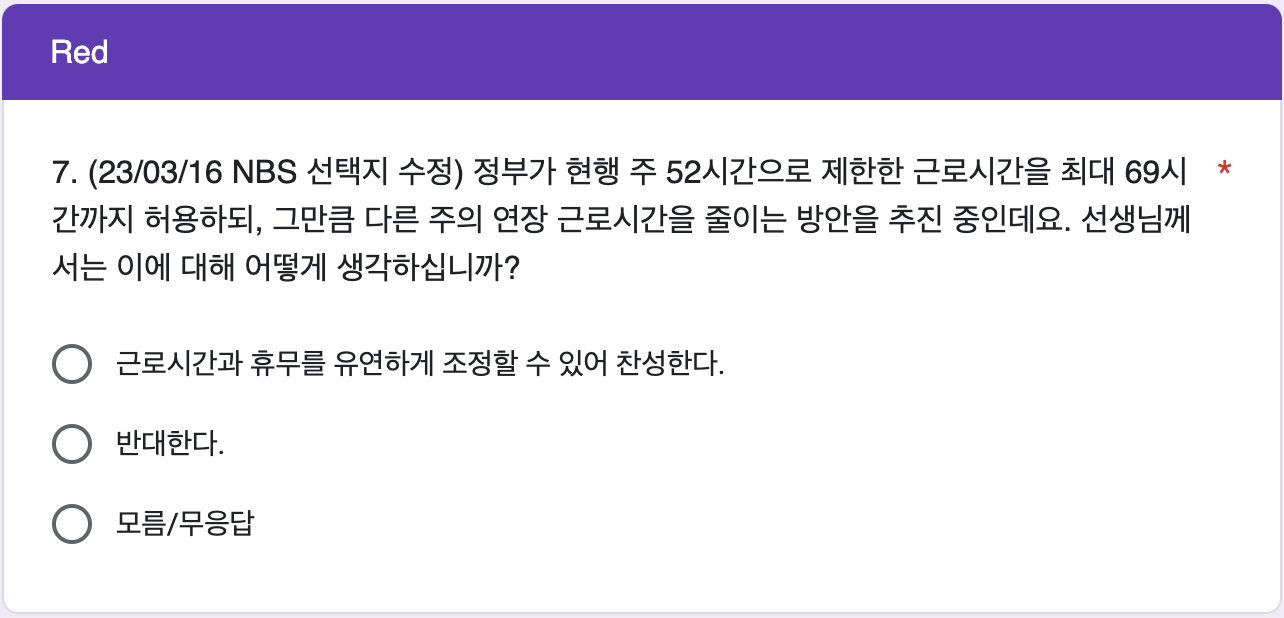
\includegraphics[width=0.67\linewidth]{./pics/Quiz240322_Q7_Red} \end{flushleft}

\begin{flushleft}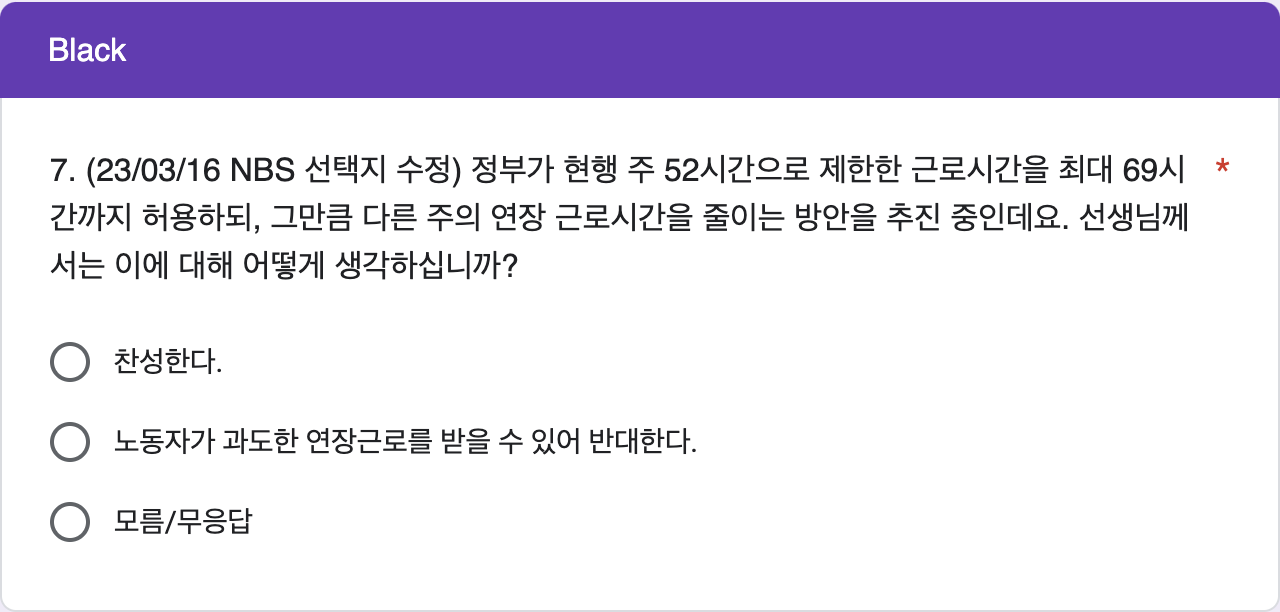
\includegraphics[width=0.67\linewidth]{./pics/Quiz240322_Q7_Black} \end{flushleft}

\subsubsection{집계}\label{uxc9d1uxacc4}

\begin{longtable}[]{@{}
  >{\raggedright\arraybackslash}p{(\linewidth - 8\tabcolsep) * \real{0.4286}}
  >{\centering\arraybackslash}p{(\linewidth - 8\tabcolsep) * \real{0.1558}}
  >{\centering\arraybackslash}p{(\linewidth - 8\tabcolsep) * \real{0.1558}}
  >{\centering\arraybackslash}p{(\linewidth - 8\tabcolsep) * \real{0.1818}}
  >{\centering\arraybackslash}p{(\linewidth - 8\tabcolsep) * \real{0.0779}}@{}}
\toprule\noalign{}
\begin{minipage}[b]{\linewidth}\raggedright
~
\end{minipage} & \begin{minipage}[b]{\linewidth}\centering
찬성한다.
\end{minipage} & \begin{minipage}[b]{\linewidth}\centering
반대한다.
\end{minipage} & \begin{minipage}[b]{\linewidth}\centering
모름/무응답
\end{minipage} & \begin{minipage}[b]{\linewidth}\centering
계
\end{minipage} \\
\midrule\noalign{}
\endhead
\bottomrule\noalign{}
\endlastfoot
\textbf{Red(찬성한다에 부연설명)} & 132 & 78 & 68 & 278 \\
\textbf{Black(반대한다에 부연설명)} & 85 & 146 & 55 & 286 \\
\textbf{계} & 217 & 224 & 123 & 564 \\
\end{longtable}

\begin{longtable}[]{@{}
  >{\raggedleft\arraybackslash}p{(\linewidth - 4\tabcolsep) * \real{0.2361}}
  >{\raggedleft\arraybackslash}p{(\linewidth - 4\tabcolsep) * \real{0.0694}}
  >{\raggedleft\arraybackslash}p{(\linewidth - 4\tabcolsep) * \real{0.2500}}@{}}
\caption{Pearson's Chi-squared test: \texttt{.}}\tabularnewline
\toprule\noalign{}
\begin{minipage}[b]{\linewidth}\raggedleft
Test statistic
\end{minipage} & \begin{minipage}[b]{\linewidth}\raggedleft
df
\end{minipage} & \begin{minipage}[b]{\linewidth}\raggedleft
P value
\end{minipage} \\
\midrule\noalign{}
\endfirsthead
\toprule\noalign{}
\begin{minipage}[b]{\linewidth}\raggedleft
Test statistic
\end{minipage} & \begin{minipage}[b]{\linewidth}\raggedleft
df
\end{minipage} & \begin{minipage}[b]{\linewidth}\raggedleft
P value
\end{minipage} \\
\midrule\noalign{}
\endhead
\bottomrule\noalign{}
\endlastfoot
32.09 & 2 & 1.076e-07 * * * \\
\end{longtable}

Q7의 Red는 주당 근로 69시간제의 도입에 찬반을 묻는 질문 중 찬성을
유도하는 부연설명을 붙였을 때 278명이 응답한 가운데 132명이
``찬성한다''는 반응을 보이고, 78명이 ``반대한다''는 반응을 보입니다.

Black은 같은 상황에서 반대를 유도하는 부연설명을 붙였을 떄 286명이
응답한 가운데 85명이 ``찬성한다''는 반응을 보이고, 146명이
``반대한다''는 반응을 보입니다.

그리고 ``모름/무응답''에 답한 인원은 Red에 68명, Black 에 55명이
응답하였습니다.

카이제곱 테스트는 이와 같은 상황에서 찬성을 유도하는 부연설명을 붙인
경우와 반대를 유도하는 부연설명을 붙인 경우에 그 응답의 차이가
통계적으로 유의하다는 것을 보여 줍니다.

카이제곱 통계량은 32.090, 자유도는 2, p-value 는 1.1e-07으로 부연설명을
어디에 붙이느냐에 따라 그 차이가 통계적으로 유의한 것으로 나왔습니다.

여기서 부연설명이 응답에 영향을 끼치지 않는다고 가정해 봅시다.

그렇다면 Red, Black 의 응답은 대부분의 Q1 \textasciitilde{} Q6 에서와
같이 랜덤화 효과에 의하여 통계적으로 유의한 차이를 보이지 않을 것입니다.

그런데 실제로 관찰된 카이제곱 통계값은 통계적으로 유의한 차이를 보여
주고 있습니다.

따라서 부연설명이 영향을 끼치지 않는다는 가정은 티당치 않은 것으로 볼
수밖에 없습니다.

이러한 논증 방식을 귀류법이라 합니다.

\subsubsection{\% 비교}\label{uxbe44uxad50}

\begin{longtable}[]{@{}
  >{\raggedright\arraybackslash}p{(\linewidth - 8\tabcolsep) * \real{0.4177}}
  >{\centering\arraybackslash}p{(\linewidth - 8\tabcolsep) * \real{0.1519}}
  >{\centering\arraybackslash}p{(\linewidth - 8\tabcolsep) * \real{0.1519}}
  >{\centering\arraybackslash}p{(\linewidth - 8\tabcolsep) * \real{0.1772}}
  >{\centering\arraybackslash}p{(\linewidth - 8\tabcolsep) * \real{0.1013}}@{}}
\toprule\noalign{}
\begin{minipage}[b]{\linewidth}\raggedright
~
\end{minipage} & \begin{minipage}[b]{\linewidth}\centering
찬성한다.
\end{minipage} & \begin{minipage}[b]{\linewidth}\centering
반대한다.
\end{minipage} & \begin{minipage}[b]{\linewidth}\centering
모름/무응답
\end{minipage} & \begin{minipage}[b]{\linewidth}\centering
계
\end{minipage} \\
\midrule\noalign{}
\endhead
\bottomrule\noalign{}
\endlastfoot
\textbf{Red(찬성한다에 부연설명)} & 47.5 & 28.1 & 24.5 & 100.0 \\
\textbf{Black(반대한다에 부연설명)} & 29.7 & 51.0 & 19.2 & 100.0 \\
\end{longtable}

찬성을 유도하는 부연설명을 붙인 Red에서 ``찬성한다''고 응답하는사람들의
백분율, 47.5(\%)은 ``반대한다''고 응답하는 사람들의 백분율, 28.1(\%)
보다 높습니다.

반면 반대를 유도하는 부연설명을 붙인 Black에서 ``찬성한다''고 응답하는
사람들의 백분율, 29.7(\%)은 ``반대한다''고 응답하는 사람들의 백분율,
51.0(\%) 보다 훨씬 적습니다.

찬성을 유도하는 부연설명을 붙이느냐, 반대를 유도하는 부연설명을
붙이느냐에 따라 반응이 달라진다는 것을 잘 알 수 있습니다.

Red 와 Black 이 워낙 차이가 나지만 전체적으로 어느 정도가
``찬성한다''하고 어느 정도가 ``반대한다''고 응답하였는지 합쳐
보겠습니다.

\subsubsection{\% 합계}\label{uxd569uxacc4}

\begin{longtable}[]{@{}
  >{\centering\arraybackslash}p{(\linewidth - 6\tabcolsep) * \real{0.1667}}
  >{\centering\arraybackslash}p{(\linewidth - 6\tabcolsep) * \real{0.1667}}
  >{\centering\arraybackslash}p{(\linewidth - 6\tabcolsep) * \real{0.1944}}
  >{\centering\arraybackslash}p{(\linewidth - 6\tabcolsep) * \real{0.1111}}@{}}
\toprule\noalign{}
\begin{minipage}[b]{\linewidth}\centering
찬성한다.
\end{minipage} & \begin{minipage}[b]{\linewidth}\centering
반대한다.
\end{minipage} & \begin{minipage}[b]{\linewidth}\centering
모름/무응답
\end{minipage} & \begin{minipage}[b]{\linewidth}\centering
계
\end{minipage} \\
\midrule\noalign{}
\endhead
\bottomrule\noalign{}
\endlastfoot
38.5 & 39.7 & 21.8 & 100.0 \\
\end{longtable}

``찬성한다''고 응답한 백분율은 Red, Black 합쳐서 38.5(\%)(으)로
'반대한다''고 응답한 백분율, 39.7(\%) 과 약간 적습니다.

그리고, 모름/무응답이 21.8(\%)로 적지 않습니다.

\subsubsection{Mosaic Plot}\label{mosaic-plot}

\pandocbounded{
\includegraphics[keepaspectratio]{quiz250324_Report_v6_files/figure-latex/unnamed-chunk-17-1.pdf}}

Mosaic Plot 은 이 집계결과를 시각적으로 잘 보여줍니다.

찬성을 유도하는 부연설명을 붙인 Red 에서 ``찬성한다''고 응답한 백분율이
높고, 반대를 유도하는 부연설명을 붙인 Black 에서 ``반대한다''고 응답한
백분율이 월등히 높은 것을 시각적으로 알 수 있습니다.

\subsection{마감 시간으로부터 제출 시간의
분포}\label{uxb9c8uxac10-uxc2dcuxac04uxc73cuxb85cuxbd80uxd130-uxc81cuxcd9c-uxc2dcuxac04uxc758-uxbd84uxd3ec}

\subsubsection{분포표}\label{uxbd84uxd3ecuxd45c}

\begin{longtable}[]{@{}
  >{\raggedright\arraybackslash}p{(\linewidth - 30\tabcolsep) * \real{0.1121}}
  >{\centering\arraybackslash}p{(\linewidth - 30\tabcolsep) * \real{0.0654}}
  >{\centering\arraybackslash}p{(\linewidth - 30\tabcolsep) * \real{0.0654}}
  >{\centering\arraybackslash}p{(\linewidth - 30\tabcolsep) * \real{0.0654}}
  >{\centering\arraybackslash}p{(\linewidth - 30\tabcolsep) * \real{0.0654}}
  >{\centering\arraybackslash}p{(\linewidth - 30\tabcolsep) * \real{0.0654}}
  >{\centering\arraybackslash}p{(\linewidth - 30\tabcolsep) * \real{0.0561}}
  >{\centering\arraybackslash}p{(\linewidth - 30\tabcolsep) * \real{0.0561}}
  >{\centering\arraybackslash}p{(\linewidth - 30\tabcolsep) * \real{0.0561}}
  >{\centering\arraybackslash}p{(\linewidth - 30\tabcolsep) * \real{0.0561}}
  >{\centering\arraybackslash}p{(\linewidth - 30\tabcolsep) * \real{0.0561}}
  >{\centering\arraybackslash}p{(\linewidth - 30\tabcolsep) * \real{0.0561}}
  >{\centering\arraybackslash}p{(\linewidth - 30\tabcolsep) * \real{0.0561}}
  >{\centering\arraybackslash}p{(\linewidth - 30\tabcolsep) * \real{0.0561}}
  >{\centering\arraybackslash}p{(\linewidth - 30\tabcolsep) * \real{0.0561}}
  >{\centering\arraybackslash}p{(\linewidth - 30\tabcolsep) * \real{0.0561}}@{}}
\caption{일 단위}\tabularnewline
\toprule\noalign{}
\begin{minipage}[b]{\linewidth}\raggedright
~
\end{minipage} & \begin{minipage}[b]{\linewidth}\centering
14일
\end{minipage} & \begin{minipage}[b]{\linewidth}\centering
13일
\end{minipage} & \begin{minipage}[b]{\linewidth}\centering
12일
\end{minipage} & \begin{minipage}[b]{\linewidth}\centering
11일
\end{minipage} & \begin{minipage}[b]{\linewidth}\centering
10일
\end{minipage} & \begin{minipage}[b]{\linewidth}\centering
9일
\end{minipage} & \begin{minipage}[b]{\linewidth}\centering
8일
\end{minipage} & \begin{minipage}[b]{\linewidth}\centering
7일
\end{minipage} & \begin{minipage}[b]{\linewidth}\centering
6일
\end{minipage} & \begin{minipage}[b]{\linewidth}\centering
5일
\end{minipage} & \begin{minipage}[b]{\linewidth}\centering
4일
\end{minipage} & \begin{minipage}[b]{\linewidth}\centering
3일
\end{minipage} & \begin{minipage}[b]{\linewidth}\centering
2일
\end{minipage} & \begin{minipage}[b]{\linewidth}\centering
1일
\end{minipage} & \begin{minipage}[b]{\linewidth}\centering
계
\end{minipage} \\
\midrule\noalign{}
\endfirsthead
\toprule\noalign{}
\begin{minipage}[b]{\linewidth}\raggedright
~
\end{minipage} & \begin{minipage}[b]{\linewidth}\centering
14일
\end{minipage} & \begin{minipage}[b]{\linewidth}\centering
13일
\end{minipage} & \begin{minipage}[b]{\linewidth}\centering
12일
\end{minipage} & \begin{minipage}[b]{\linewidth}\centering
11일
\end{minipage} & \begin{minipage}[b]{\linewidth}\centering
10일
\end{minipage} & \begin{minipage}[b]{\linewidth}\centering
9일
\end{minipage} & \begin{minipage}[b]{\linewidth}\centering
8일
\end{minipage} & \begin{minipage}[b]{\linewidth}\centering
7일
\end{minipage} & \begin{minipage}[b]{\linewidth}\centering
6일
\end{minipage} & \begin{minipage}[b]{\linewidth}\centering
5일
\end{minipage} & \begin{minipage}[b]{\linewidth}\centering
4일
\end{minipage} & \begin{minipage}[b]{\linewidth}\centering
3일
\end{minipage} & \begin{minipage}[b]{\linewidth}\centering
2일
\end{minipage} & \begin{minipage}[b]{\linewidth}\centering
1일
\end{minipage} & \begin{minipage}[b]{\linewidth}\centering
계
\end{minipage} \\
\midrule\noalign{}
\endhead
\bottomrule\noalign{}
\endlastfoot
\textbf{Red} & 71 & 15 & 13 & 4 & 10 & 3 & 6 & 46 & 20 & 22 & 14 & 20 &
16 & 18 & 278 \\
\textbf{Black} & 71 & 14 & 7 & 7 & 11 & 4 & 6 & 50 & 20 & 14 & 12 & 24 &
17 & 29 & 286 \\
\textbf{계} & 142 & 29 & 20 & 11 & 21 & 7 & 12 & 96 & 40 & 36 & 26 & 44
& 33 & 47 & 564 \\
\end{longtable}

분포표로부터 두 가지 문제를 살펴보겠습니다.

첫째, 날마다 고르게 제출하는가?

둘째, Red, Black 간에 통게적으로 유의한 차이가 있는가?

각 문제를 살펴보기 위해서는 분포표의 일부분을 대상으로 카이제곱 테스트를
수행합니다.

\subsubsection{날마다 고르게
제출하는가?}\label{uxb0a0uxb9c8uxb2e4-uxace0uxb974uxac8c-uxc81cuxcd9cuxd558uxb294uxac00}

\begin{longtable}[]{@{}
  >{\centering\arraybackslash}p{(\linewidth - 26\tabcolsep) * \real{0.0787}}
  >{\centering\arraybackslash}p{(\linewidth - 26\tabcolsep) * \real{0.0787}}
  >{\centering\arraybackslash}p{(\linewidth - 26\tabcolsep) * \real{0.0787}}
  >{\centering\arraybackslash}p{(\linewidth - 26\tabcolsep) * \real{0.0787}}
  >{\centering\arraybackslash}p{(\linewidth - 26\tabcolsep) * \real{0.0787}}
  >{\centering\arraybackslash}p{(\linewidth - 26\tabcolsep) * \real{0.0674}}
  >{\centering\arraybackslash}p{(\linewidth - 26\tabcolsep) * \real{0.0674}}
  >{\centering\arraybackslash}p{(\linewidth - 26\tabcolsep) * \real{0.0674}}
  >{\centering\arraybackslash}p{(\linewidth - 26\tabcolsep) * \real{0.0674}}
  >{\centering\arraybackslash}p{(\linewidth - 26\tabcolsep) * \real{0.0674}}
  >{\centering\arraybackslash}p{(\linewidth - 26\tabcolsep) * \real{0.0674}}
  >{\centering\arraybackslash}p{(\linewidth - 26\tabcolsep) * \real{0.0674}}
  >{\centering\arraybackslash}p{(\linewidth - 26\tabcolsep) * \real{0.0674}}
  >{\centering\arraybackslash}p{(\linewidth - 26\tabcolsep) * \real{0.0674}}@{}}
\toprule\noalign{}
\begin{minipage}[b]{\linewidth}\centering
14일
\end{minipage} & \begin{minipage}[b]{\linewidth}\centering
13일
\end{minipage} & \begin{minipage}[b]{\linewidth}\centering
12일
\end{minipage} & \begin{minipage}[b]{\linewidth}\centering
11일
\end{minipage} & \begin{minipage}[b]{\linewidth}\centering
10일
\end{minipage} & \begin{minipage}[b]{\linewidth}\centering
9일
\end{minipage} & \begin{minipage}[b]{\linewidth}\centering
8일
\end{minipage} & \begin{minipage}[b]{\linewidth}\centering
7일
\end{minipage} & \begin{minipage}[b]{\linewidth}\centering
6일
\end{minipage} & \begin{minipage}[b]{\linewidth}\centering
5일
\end{minipage} & \begin{minipage}[b]{\linewidth}\centering
4일
\end{minipage} & \begin{minipage}[b]{\linewidth}\centering
3일
\end{minipage} & \begin{minipage}[b]{\linewidth}\centering
2일
\end{minipage} & \begin{minipage}[b]{\linewidth}\centering
1일
\end{minipage} \\
\midrule\noalign{}
\endhead
\bottomrule\noalign{}
\endlastfoot
142 & 29 & 20 & 11 & 21 & 7 & 12 & 96 & 40 & 36 & 26 & 44 & 33 & 47 \\
\end{longtable}

\begin{longtable}[]{@{}
  >{\raggedleft\arraybackslash}p{(\linewidth - 4\tabcolsep) * \real{0.2361}}
  >{\raggedleft\arraybackslash}p{(\linewidth - 4\tabcolsep) * \real{0.0694}}
  >{\raggedleft\arraybackslash}p{(\linewidth - 4\tabcolsep) * \real{0.2500}}@{}}
\caption{Chi-squared test for given probabilities:
\texttt{.}}\tabularnewline
\toprule\noalign{}
\begin{minipage}[b]{\linewidth}\raggedleft
Test statistic
\end{minipage} & \begin{minipage}[b]{\linewidth}\raggedleft
df
\end{minipage} & \begin{minipage}[b]{\linewidth}\raggedleft
P value
\end{minipage} \\
\midrule\noalign{}
\endfirsthead
\toprule\noalign{}
\begin{minipage}[b]{\linewidth}\raggedleft
Test statistic
\end{minipage} & \begin{minipage}[b]{\linewidth}\raggedleft
df
\end{minipage} & \begin{minipage}[b]{\linewidth}\raggedleft
P value
\end{minipage} \\
\midrule\noalign{}
\endhead
\bottomrule\noalign{}
\endlastfoot
433.4 & 13 & 1.915e-84 * * * \\
\end{longtable}

날마다 고르게 제출하는지 알아 보았습니다.

분포표의 ``계''행에서 '계'열을 제외하고 카이제곱테스트를 수행합니다.

분포표 만으로도 쉽게 파악할 수 있지만 카이제곱테스트가 명확히 해 줍니다.

카이제곱 통계량은 433.43, 자유도는 13.00, p-value 는 1.9e-84 이므로 결코
고르게 제출한다고 말할 수 없습니다.

막대그래프로 살펴 보겠습니다.

\subsubsection{막대그래프}\label{uxb9c9uxb300uxadf8uxb798uxd504}

\pandocbounded{
\includegraphics[keepaspectratio]{quiz250324_Report_v6_files/figure-latex/unnamed-chunk-20-1.pdf}}

막대그래프는 총 제출인원 564(명) 중에 142(명), 25(\%)가 마감일에 몰리는
것을 명확히 보여주고 있습니다.

\subsubsection{Red, Black 간에
닮았는가?}\label{red-black-uxac04uxc5d0-uxb2eeuxc558uxb294uxac00}

\begin{longtable}[]{@{}
  >{\raggedright\arraybackslash}p{(\linewidth - 28\tabcolsep) * \real{0.1188}}
  >{\centering\arraybackslash}p{(\linewidth - 28\tabcolsep) * \real{0.0693}}
  >{\centering\arraybackslash}p{(\linewidth - 28\tabcolsep) * \real{0.0693}}
  >{\centering\arraybackslash}p{(\linewidth - 28\tabcolsep) * \real{0.0693}}
  >{\centering\arraybackslash}p{(\linewidth - 28\tabcolsep) * \real{0.0693}}
  >{\centering\arraybackslash}p{(\linewidth - 28\tabcolsep) * \real{0.0693}}
  >{\centering\arraybackslash}p{(\linewidth - 28\tabcolsep) * \real{0.0594}}
  >{\centering\arraybackslash}p{(\linewidth - 28\tabcolsep) * \real{0.0594}}
  >{\centering\arraybackslash}p{(\linewidth - 28\tabcolsep) * \real{0.0594}}
  >{\centering\arraybackslash}p{(\linewidth - 28\tabcolsep) * \real{0.0594}}
  >{\centering\arraybackslash}p{(\linewidth - 28\tabcolsep) * \real{0.0594}}
  >{\centering\arraybackslash}p{(\linewidth - 28\tabcolsep) * \real{0.0594}}
  >{\centering\arraybackslash}p{(\linewidth - 28\tabcolsep) * \real{0.0594}}
  >{\centering\arraybackslash}p{(\linewidth - 28\tabcolsep) * \real{0.0594}}
  >{\centering\arraybackslash}p{(\linewidth - 28\tabcolsep) * \real{0.0594}}@{}}
\toprule\noalign{}
\begin{minipage}[b]{\linewidth}\raggedright
~
\end{minipage} & \begin{minipage}[b]{\linewidth}\centering
14일
\end{minipage} & \begin{minipage}[b]{\linewidth}\centering
13일
\end{minipage} & \begin{minipage}[b]{\linewidth}\centering
12일
\end{minipage} & \begin{minipage}[b]{\linewidth}\centering
11일
\end{minipage} & \begin{minipage}[b]{\linewidth}\centering
10일
\end{minipage} & \begin{minipage}[b]{\linewidth}\centering
9일
\end{minipage} & \begin{minipage}[b]{\linewidth}\centering
8일
\end{minipage} & \begin{minipage}[b]{\linewidth}\centering
7일
\end{minipage} & \begin{minipage}[b]{\linewidth}\centering
6일
\end{minipage} & \begin{minipage}[b]{\linewidth}\centering
5일
\end{minipage} & \begin{minipage}[b]{\linewidth}\centering
4일
\end{minipage} & \begin{minipage}[b]{\linewidth}\centering
3일
\end{minipage} & \begin{minipage}[b]{\linewidth}\centering
2일
\end{minipage} & \begin{minipage}[b]{\linewidth}\centering
1일
\end{minipage} \\
\midrule\noalign{}
\endhead
\bottomrule\noalign{}
\endlastfoot
\textbf{Red} & 71 & 15 & 13 & 4 & 10 & 3 & 6 & 46 & 20 & 22 & 14 & 20 &
16 & 18 \\
\textbf{Black} & 71 & 14 & 7 & 7 & 11 & 4 & 6 & 50 & 20 & 14 & 12 & 24 &
17 & 29 \\
\end{longtable}

\begin{longtable}[]{@{}
  >{\raggedleft\arraybackslash}p{(\linewidth - 4\tabcolsep) * \real{0.2361}}
  >{\raggedleft\arraybackslash}p{(\linewidth - 4\tabcolsep) * \real{0.0694}}
  >{\raggedleft\arraybackslash}p{(\linewidth - 4\tabcolsep) * \real{0.1389}}@{}}
\caption{Pearson's Chi-squared test: \texttt{.}}\tabularnewline
\toprule\noalign{}
\begin{minipage}[b]{\linewidth}\raggedleft
Test statistic
\end{minipage} & \begin{minipage}[b]{\linewidth}\raggedleft
df
\end{minipage} & \begin{minipage}[b]{\linewidth}\raggedleft
P value
\end{minipage} \\
\midrule\noalign{}
\endfirsthead
\toprule\noalign{}
\begin{minipage}[b]{\linewidth}\raggedleft
Test statistic
\end{minipage} & \begin{minipage}[b]{\linewidth}\raggedleft
df
\end{minipage} & \begin{minipage}[b]{\linewidth}\raggedleft
P value
\end{minipage} \\
\midrule\noalign{}
\endhead
\bottomrule\noalign{}
\endlastfoot
7.798 & 13 & 0.8565 \\
\end{longtable}

제출시간의 분포가 Red, Black 간에 닮았는지 알아 보았습니다.

이번에는 분포표의 첫번째와 두번째 행, '계'열을 제외한 나머지 열에 대해서
카이제곱테스트를 수행합니다.

카이제곱 통계량은 7.798, 자유도는 13, p-value 는 0.8565 이므로 제출
시간의 분포는 Red, Black 간에 통계적으로 유의한 차이가 관찰되지
않습니다.

이 사실을 Mosaic Plot 을 이용하여 시각적으로 살펴보겠습니다.

닮았다고 느껴지나요?

\subsubsection{Mosaic Plot}\label{mosaic-plot-1}

\pandocbounded{
\includegraphics[keepaspectratio]{quiz250324_Report_v6_files/figure-latex/unnamed-chunk-22-1.pdf}}

\end{document}
